% LaTeX mintafájl szakdolgozat és diplomamunkáknak az
% SZTE Informatikai Tanszekcsoportja által megkövetelt
% formai követelményeinek megvalósításához
% Modositva: 2011.04.28 Nemeth L. Zoltan
% A fájl használatához szükséges a magyar.ldf 2005/05/12 v1.5-ös vagy későbbi verziója
% ez letölthető a http://www.math.bme.hu/latex/ weblapról, a magyar nyelvű szedéshez
% Hasznos információk, linekek, LaTeX leirasok a www.latex.lap.hu weboldalon vannak.
%


\documentclass[12pt, a4paper]{report}
%Magyar nyelvi támogatás (Babel 3.7 vagy későbbi kell!)
\usepackage[utf8]{inputenc}
\usepackage{t1enc}
\usepackage[magyar]{babel}
% A formai kovetelmenyekben megkövetelt Times betűtípus hasznalata:
\usepackage{times}
\usepackage{url}
\usepackage{indentfirst}

%Az AMS csomagjai
\usepackage{amsmath}
\usepackage{amssymb}
\usepackage{amsthm}

%A fejléc láblécek kialakításához:
\usepackage{fancyhdr}

%Természetesen további csomagok is használhatók,
%például ábrák beillesztéséhez a graphix és a psfrag,
%ha nincs rájuk szükség természetesen kihagyhatók.
\usepackage{graphicx}
\usepackage{psfrag}
%Define the listing package
\usepackage{listings} %code highlighter
\usepackage{color} %use color
\definecolor{mygreen}{rgb}{0,0.6,0}
\definecolor{mygray}{rgb}{0.8,0.8,0.8}
\definecolor{mymauve}{rgb}{0.58,0,0.82}

%Customize a bit the look
\lstset{ %
	backgroundcolor=\color{white}, % choose the background color; you must add \usepackage{color} or \usepackage{xcolor}
	basicstyle=\footnotesize, % the size of the fonts that are used for the code
	breakatwhitespace=false, % sets if automatic breaks should only happen at whitespace
	breaklines=true, % sets automatic line breaking
	captionpos=t, % sets the caption-position to bottom
	commentstyle=\color{mygreen}, % comment style
	deletekeywords={...}, % if you want to delete keywords from the given language
	escapeinside={\%*}{*)}, % if you want to add LaTeX within your code
	extendedchars=true, % lets you use non-ASCII characters; for 8-bits encodings only, does not work with UTF-8
	frame=none, % adds a frame around the code
	keepspaces=true, % keeps spaces in text, useful for keeping indentation of code (possibly needs columns=flexible)
	keywordstyle=\color{blue}, % keyword style
	% language=Octave, % the language of the code
	morekeywords={*,...}, % if you want to add more keywords to the set
	numbers=left, % where to put the line-numbers; possible values are (none, left, right)
	numbersep=5pt, % how far the line-numbers are from the code
	numberstyle=\tiny\color{mygray}, % the style that is used for the line-numbers
	rulecolor=\color{black}, % if not set, the frame-color may be changed on line-breaks within not-black text (e.g. comments (green here))
	showspaces=false, % show spaces everywhere adding particular underscores; it overrides 'showstringspaces'
	showstringspaces=false % underline spaces within strings only
	showtabs=false, % show tabs within strings adding particular underscores
	stepnumber=1, % the step between two line-numbers. If it's 1, each line will be numbered
	stringstyle=\color{mymauve}, % string literal style
	tabsize=2, % sets default tabsize to 2 spaces
	title=\lstname % show the filename of files included with \lstinputlisting; also try caption instead of title
}
%END of listing package%

\definecolor{darkgray}{rgb}{.4,.4,.4}
\definecolor{purple}{rgb}{0.65, 0.12, 0.82}

%define Javascript language
\lstdefinelanguage{JavaScript}{
	keywords={typeof, new, true, false, catch, function, return, null, catch, switch, var, if, in, while, do, else, case, break, const, var, let},
	keywordstyle=\color{blue}\bfseries,
	ndkeywords={class, export, boolean, throw, implements, import, this},
	ndkeywordstyle=\color{darkgray}\bfseries,
	identifierstyle=\color{black},
	sensitive=false,
	comment=[l]{//},
	morecomment=[s]{/*}{*/},
	commentstyle=\color{purple}\ttfamily,
	stringstyle=\color{red}\ttfamily,
	morestring=[b]',
	morestring=[b]"
}

\lstset{
	language=JavaScript,
	extendedchars=true,
	basicstyle=\footnotesize\ttfamily,
	showstringspaces=false,
	showspaces=false,
	numbers=left,
	numberstyle=\footnotesize,
	numbersep=9pt,
	tabsize=2,
	breaklines=true,
	showtabs=false,
	captionpos=t
}

%tetelszerű környezetek definiálhatók, ezek most fejezetenkent egyutt szamozodnak, pl.
\newtheorem{tet}{tetel}[chapter]
\newtheorem{defi}[tet]{Definíció}
\newtheorem{lemma}[tet]{Lemma}
\newtheorem{áll}[tet]{Állítás}
\newtheorem{köv}[tet]{Következmény}

%Ha a megjegyzések és a példak szövegét nem akarjuk dőlten szedni, akkor
%az alábbi parancs után kell őket definiální:
\theoremstyle{definition}
\newtheorem{megj}[tet]{Megjegyzés}
\newtheorem{pld}[tet]{Példa}

%Margók:
\hoffset -1in
\voffset -1in
\oddsidemargin 35mm
\textwidth 150mm
\topmargin 15mm
\headheight 10mm
\headsep 5mm
\textheight 237mm


\begin{document}
	
	%A FEJEZETEK KEZDŐOLDALAINAK FEJ ES LÁBLÉCE:
	%a plain oldalstílust kell átdefiniálni, hogy ott ne legyen fejléc:
	\fancypagestyle{plain}{%
		%ez mindent töröl:
		\fancyhf{}
		% a láblécbe jobboldalra kerüljön az oldalszám:
		\fancyfoot[R]{\thepage}
		%elválasztó vonal sem kell:
		\renewcommand{\headrulewidth}{0pt}
	}
	
	%A TÖBBI OLDAL FEJ ÉS LÁBLÉCE:
	\pagestyle{fancy}
	\fancyhf{}
	\fancyhead[L]{Platformfüggetlen 2D játék fejlesztése Phaser használatával}
	\fancyfoot[R]{\thepage}
	
	
	%A címoldalra se fej- se lábléc nem kell:
	\thispagestyle{empty}
	
	\begin{center}
		\vspace*{1cm}
		{\Large\bf Szegedi Tudományegyetem}
		
		\vspace{0.5cm}
		
		{\Large\bf Informatikai Intézet}
		
		\vspace*{3.8cm}
		
		
		{\LARGE\bf Platformfüggetlen 2D játék fejlesztése Phaser használatával. }
		
		
		\vspace*{3.6cm}
		
		{\Large Diplomamunka}
		% vagy {\Large Szakdolgozat}
		
		\vspace*{4cm}
		
		%Értelemszerűen megváltoztatandó:
		{\large
			\begin{tabular}{c@{\hspace{4cm}}c}
				\emph{Készítette:}     &\emph{Témavezető:}\\
				\bf{Pigniczki Mercédesz Tamara}  &\bf{Dr. Antal Gábor}\\
				üzemmérnök-informatika szakos     &egyetemi docens\\
				hallgató&
			\end{tabular}
		}
		
		\vspace*{2.3cm}
		
		{\Large
			Szeged
			\\
			\vspace{2mm}
			2023
		}
	\end{center}
	
	%A tartalomjegyzék:
	\tableofcontents
	%1.5 sorköz
	\linespread{1.5}\selectfont
	
	%A \chapter* parancs nem ad a fejezetnek sorszámot
	\chapter*{Feladatkiírás}
	%A tartalomjegyzékben mégis szerepeltetni kell, mint szakasz(section) szerepeljen:
	\addcontentsline{toc}{section}{Feladatkiírás}

	A témavezető által megfogalmazott feladatkiírás. Önálló oldalon szerepel.

	\chapter*{Tartalmi összefoglaló}
	\addcontentsline{toc}{section}{Tartalmi összefoglaló}
	Téma megnevezése:
	
	Megadott feladat megfogalmazása:
	
	
	Megoldási mód:
	
	
	Alkalmazott eszközök, módszerek:
	
	
	Elért eredmények:
	
	
	Kulcsszavak:
	A tartalmi összefoglalónak tartalmaznia kell (rövid, legfeljebb egy oldalas, összefüggő megfogalmazásban)
	a következőket: a téma megnevezése, a megadott feladat megfogalmazása - a feladatkiíráshoz viszonyítva-,
	a megoldási mód, az alkalmazott eszközök, módszerek, az elért eredmények, kulcsszavak (4-6 darab).

	Az összefoglaló nyelvének meg kell egyeznie a dolgozat nyelvével. Ha a dolgozat idegen nyelven készül,
	magyar nyelvű tartalmi összefoglaló készítése is kötelező (külön lapon), melynek terjedelmét a TVSZ szabályozza.


	\chapter*{Bevezetés}
	\addcontentsline{toc}{section}{Bevezetés}
	A videojátékok napjainkban szinte minden korosztály életében szerepet játszik, legyen szó a fiatalabb generációról vagy akár idősebbről. A játékfejlesztést története egészen az 50-es évek elejére nyúlik vissza, ugyanis a legelső számítógépes játékot 1952-ben mutatták be az EDSAC számítógépen. A játék, egy kétszemélyes játék, ahol egy 3x3-as négyzetrácson kell "X" és "O" jeleket elhelyezni, úgy, hogy egy sorban vagy oszlopban összegyűljön az összes jel. Ezt a játékot manapság mindenki úgy ismeri, hogy Tic-tac-toe.
	
	Az első játék megjelenését követően a videojátékok robbanásszerűen elkezdtek fejlődni. Míg a 60-as években egyszerű ügyességi és reakcióteszteken alapuló játékok voltak csak elérhetőek, a 90-es évekre már otthon játszható 3D-s játékok is megjelentek. Az igazi nagy áttörés a 2000-es évek elején történt, amikor megjelentek az online, mobil és konzol játékok, amelyek nagy hatást gyakoroltak a játékfejlesztésre és az egész játékiparra.
	
	A mai kor technológiájának köszönhetően szinte mindenki rendelkezik legalább egy olyan eszközzel, amely használható játékra. Egy 2023-es kutatás szerint 3.09 milliárd ember játszik videojátékokkal és a játékpiac bevétele elérte az 197.11 milliárd dollárt. A felhasználók száma 1 milliárd fővel nőtt ez elmúlt hét  évben, és minden évben átlagosan 150 millió fővel nő. A játékosok többsége férfi, 2006-ban csupán a játékosok 38\%-a volt nő, mostanra ez az arány 45\%-ra nőtt. A játékosok 80\%-a elmúlt 18 éves, de 20\%-uk még fiatalkorú. A kutatás azt is megállapította, hogy az emberek nagy része szabadidős tevékenységként és kikapcsolódásként tekint a játékokra, viszont csak 38\%-uk használja logikát fejlesztő okok miatt.
	
	Szakdolgozati témámnak azért választottam a játékfejlesztést, mert ebben látom a lehetőséget arra, hogy kreatív és egyedi szoftvert tudjak létrehozni, aminek használata örömet okoz az emberek számára. A programozás mellett szívesen fordítok időt grafikai munkák elkészítésére, ezért a játékfejlesztés egy remek kihívás volt a számomra, mint megjelenítési, mind játéklogikai szempontból is. A játék fejlesztéséhez a TypeScript nyelvet választottam Phaser keretrendszer használatával, mivel a tanulmányaim során leginkább a szkript nyelvek tetszettek a legjobban. A keretrendszer lehetővé teszi, hogy elkészítsünk egy játékot webes és mobil felületre is. Ez azért fontos, mert azok a játékok amelyek platformfüggetlenek, növelik a játéklátogatottságát, mivel a felhasználók széles körben tudnak hozzá jutni. Ilyen játékok pl.: "Angry Birds", "Candy Crush", "Among us", melyek manapság a legnépszerűbb játékok köré tartoznak.
	
	
	\chapter{Felhasznált technológiák bemutatása}
	Ebben a fejezetben bemutatom azokat a programozási technikákat, amelyeket használtam a fejlesztés során. Ismertetem az általam használt nyelveket, keretrendszereket és egyéb eszközöket.
	\section{A szkript nyelvek alkalmazása játékfejlesztésben}
	A játékfejlesztés területén a szkript nyelvek használata széles körben elterjedt. 
	Ezek olyan magas szintű programozási nyelvek, amelyek lehetővé teszik, hogy a programot egyszerűbb és gyorsabb módon fejlesszük, az alacsonyabb szintű nyelvekhez képest.
	
	\subsection{HTML5}
	A HTML5 egy átdolgozottabb változata a HTML (HyperText Markup Language) szabványosított leíró nyelvnek, melyet weboldalak létrehozására és strukturálására használnak. Lehetővé teszi a szövegek, képek, hivatkozások stb. létrehozását. A HTML5 megalkotásának fő célja a platformfüggetlenség támogatása volt, ugyanis reszponzív és mobiltelefonokon kevesebb sávszélesség használat szükséges hozzá a HTML-hez lépest, ami gyorsabb oldalbetöltést eredményez, ezáltal javítja a felhasználói élmény.
	
	\subsection{JavaScript}
	A JavaScript egy könnyen tanulható, objektum orientált programozási nyelv, amelyet eredetileg 1996-ban hoztak létre a dinamikus weboldalak készítésére. Az addig statikus weboldalak csak információkat közvetítettek, azonban a JavaScript megjelenésével az adatbázis-vezérelt weboldalak is létrejöhettek, amelyek lehetővé teszik az adatok valós idejű generálását egy adott felhasználó számára. Ezáltal a JavaScript nagyban hozzájárult a webes alkalmazások fejlődéséhez és az interaktívabb felhasználói élmények megteremtéséhez.
	
	\subsection{TypeScript}
	A TypeScript egy objektum-orientált programozási nyelv, amelyet a JavaScript kibővítéseként és továbbgondolásaként hoztak létre. Alapvetően a TypeScript tudja használni ugyanazt a kódot, mint a JavaScript nyelv. Azaz egy működő JavaScript kódot lefuttathatunk TypeSctipt kódként, azonban a TypeScript statikus típusellenőrzést végez, ami azt jelenti, hogy ha a kódunk hibás típusokat tartalmaz, akkor fordítási időben hibát dobhat, azonban a futási időben a kód viselkedése nem fog változni.
	A két nyelv nagyon hasonló azonban vannak fontos különbségek:
	\begin{itemize}
		\item Futtatás: A TypeScript forráskódját először le kell fordítani JavaScript forráskóddá, mielőtt futtatható lenne a böngészőben.
		\item Típusrendszer: Míg a JavaScript egy dinamikus nyelv, amelyben a változók típusát nem kell előre meghatározni, addig a TypeScript statikus típusellenőrzést végez, ami segít a hibák korai felfedezésében. Tehát a fejlesztőknek előre meg kell határozniuk a változók, függvények és objektumok típusát.
		\item Objektum-orientáltság: A TypeScript erősebb objektum-orientáltságot biztosít, ugyanis több objektum-orientált funkcióval rendelkezik, mint a JavaScript, például a dekorátorokkal és az interfészekkel.
	\end{itemize}
	A TypeScript elterjedt használata a statikus típusellenőrzésnek köszönhető, ugyanis fejlesztők gyakran hajlamosak voltak hibás típusokat használni a JavaScript kódjukban, ami sokszor problémát okozott. Azonban típusellenőrzés miatt ezeket a hibákat már korábban észrevehetjük és megelőzhetjük, ami gyorsítja a fejlesztési folyamatot, ezért alkalmasabb a nagyobb projektek készítésénél. Összességében a TypeScript egy hatékonyabb és megbízhatóbb szkriptnyelv a dinamikus típusú JavaScripthez képest. 
	
	\subsection{PhaserJS}
	A PhaserJS egy olyan játékfejlesztő keretrendszer, amely könnyen megtanulható és kifejezetten 2D játékok létrehozására lett tervezve. A nyelv lehetővé teszik a HTML5 alapú játékok hatékony fejlesztését, amely során JavaScript és a TypeScript nyelv is egyaránt használható. 
	
	A keretrendszerének kiválasztásakor több szempontot is figyelemebe vettem. Mivel még nem készítettem játékot ezért a nyelv tanulhatósága egy fontos szempont volt. A keretrendszer rendelkezik hivatalos, jól értelmezhető dokumentációval, valamint egy aktív és segítőkész fejlesztői közösséggel, akik folyamatosan támogatják egymást a munkájukban.
	
	Ezen felül a keretrendszer rengeteg olyan funkciót kínál, amelyek szükségesek egy játék fejlesztéséhez. Ezek közé tartoznak az animációk, hangeffektek, az egérrel és érintőképernyővel való irányítás valamint a fizikai interakciók, azaz lehetővé teszi, hogy az objektumok reagáljanak egymásra. A PhaserJS előnye, hogy rendkívül rugalmas, és sokféle játékot lehet vele készíteni, beleértve az egyszerű arcade játékoktól a stratégiai játékokon át az interaktív oktatójátékokig szinte bármilyen játékot. Ezen kívül sokféle megjelenési stílust támogat, legyen ez rajzfilmszerű, retro, klasszikus pixel art vagy akár modern látványvilág.
	
	A keretrendszer azért is nagyon népszerű, mert platformfüggetlen, így ugyanazon kód alapján készíthetünk játékot webre, iOS-re és Androidra egyaránt.
	
	A játék fejlesztése során három alapvető függvényt használhatunk:
		\begin{itemize}
		\item preload(): A játékelemek előzetes betöltésére szolgál, amik lehetnek képek, videók, hangok vagy bármilyen fájl ami a játék megjelenítésért felelős. Ez a függvény hívódik meg először azért, hogy a játék indítása előtt minden elem betöltődjön, ezért ez rendkívül fontos, ugyanis ha a betöltési idő hosszú a felhasználó csak egy fekete képernyőt lát, ami ront a játékélményen.
		\item create(): A játék inicializálásához szükséges objektumok és elemek létrehozására szolgál. Itt hozzuk létre a játékteret, azaz a pályát, hátteret, a játékosokat és az ellenfeleket, illetve azok tulajdonságait, mint a sebesség, a pozíció és a méret.
		\item update(): A játék az objektumainak állapotának frissítésére szolgál. A függvény minden egyes képkocka után le fut, és frissíti az objektumok állapotait az új képkocka szerint. A függvényben létrehozott kód határozza meg a játék logikáját, például azt, hogy mi történjen, ha a játékos megnyomja a billentyűt, mikor induljon el egy adott animáció, vagy akár az ütközésvizsgálatokat.
	\end{itemize}
	A PhaserJS számos beépített osztállyal rendelkezik. Az általam felhasználtak közül ezek a legfontosabbak:
	\begin{itemize}
	\item GameObject: Az összes játékban megjelenő objektum ebből az osztályból származik.
	\item Game: A játékmotor, amely felelős a játék indításáért, az objektumok létrehozásáért, valamint felelős a játékmenet kezeléséért.
	\item Config: Itt adhatók meg a játék konfigurációs beállításai, mint például a képernyő mérete, gravitáció erőssége, fizikai motor típusa és működése és a játék képernyői.
	\item Scene: Ez az osztály kezeli a különböző képernyőket, és itt találhatók a képernyőn megjelenő objektumok.
	\item Camera: A Camera osztály lehetővé teszi a játéktér mozgatását és nagyítását.
	\item Sprite: Egy olyan objektum, amely képes megjeleníteni a játékelemet a képernyőn.
	\item Group: Az objektumok csoportos kezelését teszi lehetővé, ezáltal egyszerre lehet őket létrehozni, módosítani vagy törölni.
	\item Arcade fizikai motor: Az alapértelmezett fizikai motor a Phaser-ben, melynek a fő célja, hogy egyszerű fizikai modelleket biztosítson 2D játékokhoz, így könnyebben használható.
	\item Matter fizikai motor: Több funkcióval rendelkező fizikai motor, ami nagyobb funkcionalitást és nagyobb pontosságot kínál a játékok fizikai szimulációjához.
	\item Overlap: Ütközésvizsgálat, mely vizsgálja az objektumok közötti átfedés.
	\item Collision: Ütközésvizsgálat, amely lehetővé teszi a játékban szereplő objektumok ütközésének észlelését és kezelését.
	\end{itemize}
	
	\subsection{TileMap}
	A Tile-Map alapú megjelenítési technika kifejezetten elterjedt a két dimenziós játékfejlesztésnél. A lényege, hogy a játékterületet úgynevezett tile-okra bontjuk, és ezeket a tile-okat a memóriában csak egyszer töltjük be, ezáltal újrafelhasználhatóvá tesszük őket a megjelenő háttérhez, így jelentős memóriamegtakarítást érhetünk el ennek a segítségével. Ezek a tile-ok egy Tileset nevű képen tárolódnak, ami az összessége ezeknek a kockáknak.
	\begin{figure}[!h]
		\centering
		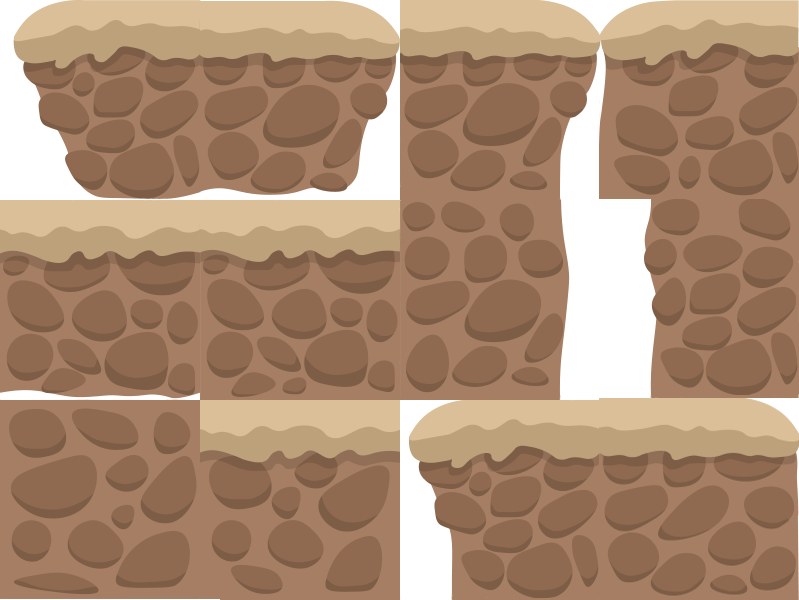
\includegraphics[width=0.4\linewidth]{./images/tile.png}
		\caption{Az általam felhasznált Tileset}
		\label{fig:tileset}
	\end{figure}
	Ahogy, a \ref{fig:tileset} ábrán látható.
	
	A szakdolgozati munkám során a Tiled nevű ingyenes és nyílt forráskódú szoftvert használtam a játék pályájának létrehozásához. A program használata során először importáltam a meglévő Tileset képemet, majd beállítottam a pálya paramétereit. Ezt követően megrajzoltam a pályát, majd objektumokat hoztam létre külön rétegekre, ezeknek megadtam a nevét, méretét és a pályán lévő helyét. Végül a program generált egy JSON fájlt a rétegekből, amelyet egyszerűen be tudtam importálni a Phaser játékomba.  
	
	
	\subsection{Webpack}
	A Webpack egy JavaScript és TypeScript modulkezelő, amely a különböző forrásfájlokat összecsomagolja egyetlen JavaScript fájlba. A szoftver elsősorban JavaScripthez készült, de támogatja a Loaderek használatát, ami lehetővé teszi, hogy a CSS és a felhasznált képek, játékelemek is becsomagolhatóak legyenek egyetlen fájlba. 
	
	A szakdolgozatom során azért volt szükség a modulkezelő használatára, mert a TypeScript kódot először le kell fordítanunk JavaScript kóddá, hogy a böngészőnk futtatni tudja. A játékom során több TypeScript fájlt is létrehoztam, ami jelentősen csökkentette a játék sebességét, a modulkezelő azonban a fájlokat egyesével átkonvertálja JavaScript fájlokká, majd ezeket egyetlen fájlba csomagolja. Ennek a módszernek a segítségével a játék gyorsabbá válik, ugyanis az összes fájl egyetlen HTTP kéréssel tölthető be. Ráadásul a felesleges kódrészleteket eltávolítja, így az alkalmazás mérete minimalizálódik, ezáltal még gyorsabb lesz a játék betöltése.
	
	\subsection{Cordova}
	A Cordova egy olyan keretrendszer, amellyel a platformfüggetlen mobil alkalmazásokat fejleszthetünk, a webes technológiák segítségével. A keretrendszer kiterjeszti a HTML és JavaScript nyújtotta lehetőségeket, hogy működjenek mobil eszközökön is. Támogatja az IOS-re valamint az Androidra, valamint a Windows Phone-ra való fejlesztést is. Az egyik legfőbb előnye, hogy úgy készíthetünk mobil alkalmazásokat, hogy nem kell ismernünk az adott platform specifikus nyelvét.
	
	A szakdolgozatom fejleszése során a Webpackg segítségével becsomagolt kódomat, a Cordova keretrendszer segítségével átalakítottam natív alkalmazásokká mobil platformra.
	\begin{figure}[!h]
		\centering
		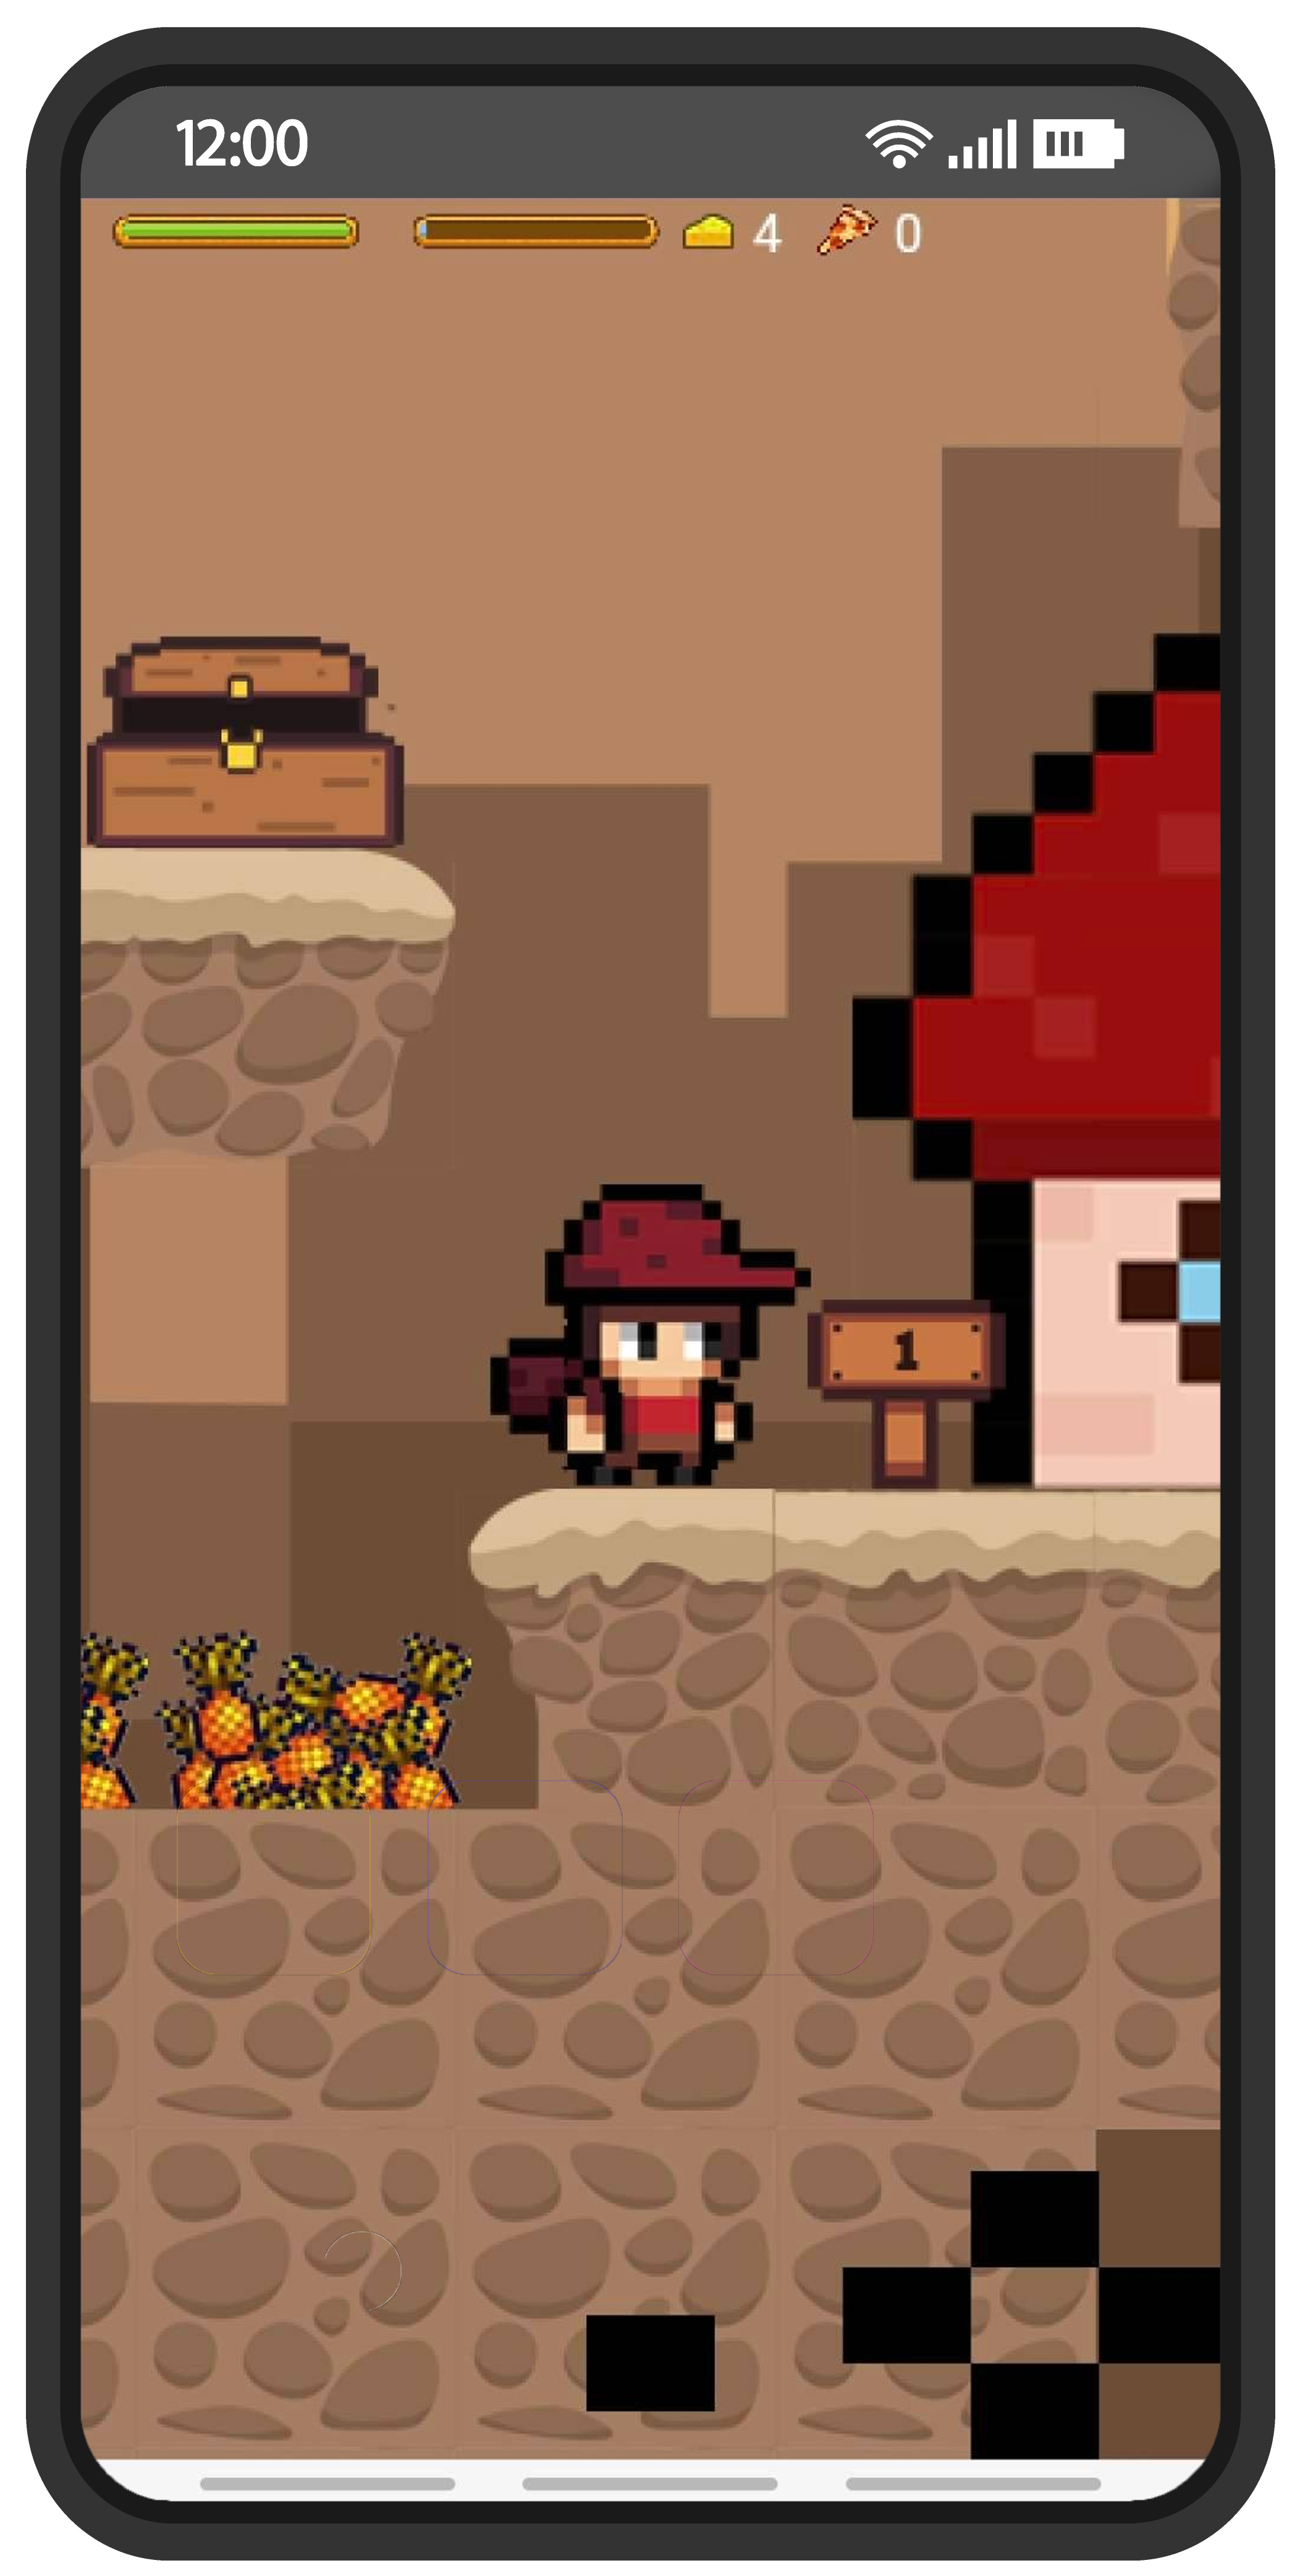
\includegraphics[width=0.20\linewidth]{./images/phone.jpg}
		\caption{Az elkészült mobil app}
		\label{fig:de}
	\end{figure}

	\section{Egyéb használt technológiák}
	A fejlesztési feladatokon túl, én készítettem el a játék grafikai elemeit, amit ebben a fejezetben mutatok be, valamint a verziókövető rendszert, amelyet a fejlesztés során használtam.
	
	\subsection{Adobe Illustrator}
	 Az Illustrator lehetővé teszi, hogy kiváló minőségű vektorgrafikus munkákat hozzunk létre, ezáltal a grafikák könnyedén skálázhatók bármilyen méretre anélkül, hogy elveszítenék az élességüket. A szoftver segítségével készítettem el a különböző grafikai tartalmakat, amelyek megjelennek a játékomban, először a pályát, majd az ezen található elemeket, végül az egyéb grafikai elemeket készítettem el.
	\begin{figure}[!h]
		\centering
		
\includegraphics[width=0.9\linewidth]{./images/characters.png}
		\caption{Az általam rajzolt karakterek}
			\label{fig:de}
	\end{figure}

	\subsection{Adobe Photoshop}
	Az Adobe Photoshop egy nagyon sokoldalú képszerkesztő és fényképfeldolgozó szoftver, amely számos eszközt tartalmaz. A szakdolgozatom során a TileSetet készítettem el a szoftver segítségével, az Illustratorban lévő grafikai elemeket felhelyeztem egy 500x500px szélességű fájlra, majd átkonvertáltam png formátumra ezeket.
	
	\subsection{Git}
	A git egy verziókezelő rendszer, amely lehetővé teszi, hogy nyomon kövessük az alkalmazásunk kódjának változtatásait a fejlesztési folyamat során. A rendszer egy úgynevezett "repository"-ban tárolja a kódbázist, amelyhez egyszerre több fejlesztő is hozzáférhet. A git számos funkcióval rendelkezik, azonban a fő funkciói, hogy ágakat tudunk létrehozni és kezelni azokat, ezekre az ágakhoz hozzá tudjuk adni a változtatásokat, majd ezeket az ágakat össze is tudjuk vonni, így teszi elérhetővé, hogy a több fejlesztő egyszerre dolgozzon. 
	
	\subsection{Firebase}
	A Firebase egy felhő alapú platform, amit a Google fejlesztett ki, lehetővé teszi az alkalmazások fejlesztését, tesztelését és üzemetetését. Egy Firebase projekthez több alkalmazás is tartozhat, például egy játék fizetős, illetve egy ingyenes verziója. Ennek következtében az erőforrások elosztott erőforrásként működnek, ezért nem történik redundáns adattárolás. 
	
	A szakdolgozatom során az adatok tárolását a Firestore adatbázis biztosította, ami lehetővé tette, hogy a játékom valós idejű adatokat szinkronizáljon az eszközök között, anélkül, hogy relációs adatbázist használna. Az adatstruktúra hierarchikus és rugalmas, az adatokat dokumentumokban tárolja, amelyek kollekciókba vannak rendezve. A dokumentumokban lehetnek alkollekciók is, így összetett beágyazott objektumokat lehet létrehozni. A lekérdezések egyszerűen megírhatók, és lehetőség van a teljes kollekció vagy alkollekciók, dokumentumokon belüli beágyazott objektumok és szűrők kombinálására.	
	
	A játékomba való autentikációt is a Firebas-el oldottam meg. A Firebase Authentication lehetővé teszi a felhasználók regisztrációját és bejelentkezését az adott alkalmazásba. A rendszer többféle bejelentkezést is biztosít, illetve biztonságosan kezeli a jelszavakat.
	
	\chapter{Saját játék tervezése}
	
	Ebben a fejezetben részletesen bemutatom az elkészült játékom szabályait és az UML diagramok tervezését. Az UML segítségével készítettem el a class diagramot és a use case diagramot, amelyek fontos előkészítő lépései voltak a játék megvalósításának. 
	
	\section{A játék megtervezése}
	A tervezési fázis során a céloknak a meghatározása volt az első lépés, majd a játék szabályrendszerét alakítottam ki, figyelembe véve a már meghatározott célokat, illetve az elképzelt játékmenetet. A tervezés során figyelembe kellett venni a választott nyelv lehetőségeit, emellett a játék különböző elemeit, például a karaktereket, a környezetet és az tárgyakat. Végül az UML tervek segítségével megterveztem a szükséges osztályokat, valamint a használati eseteket. A folyamatok során a cél az volt, hogy alaposan előkészítsem a játékot a megvalósítási fázisra.
		
	\subsection{Célok}
	A fő célkitűzésem egy 2D platformjáték tervezése és készítése volt. Az volt a célom, hogy a játék visszarepítse a felhasználókat a régi webes játékok világába. Valamint egy kiváló játékélményt nyújtson a játékosok számára, amelyet egyaránt élvezhetnek webes és mobilos környezetben is. A játék egyjátékos módja mellett lehetőséget szerettem volna adni a felhasználóknak a regisztrációra és emellett az eredmények nyilvántartására. 
	
	\subsection{Szabályok}
	A játék egy pizzafutár szerepébe helyezi a játékosokat, akinek az a feladata, hogy végigmenjen a pályán. Az útját azonban ajtók zárják el, amelyek kinyitásához pizzákat kell szállítani. A pizzák előállításához pedig paradicsomot, bacont, sajtot és kolbászt lehet felhasználni, amelyeket ládákból lehet kivenni a pálya különböző pontjain. Azonban az út során az ellenségek megtámadják a játékost, amely csökkenti az életerejét. Az ellenségeknek különböző látótávolságuk van, és ha a játékos a látótávolságukba kerül, megtámadják. A játék során három típusú ellenséggel találkozhatunk:
	\begin{itemize} 
		\item Ninja: a látótávolsága kicsi, a mozgása gyors, és ha eléri a játékost, sebzést okoz neki; 
		\item Mama: közepes látótávolsága van, lassú a mozgása, és ha hozzáérünk, eltávolít egy élelmiszert a begyűjtöttek közül; 
		\item Vadász: nagy látótávolsága van, és messzebbről is képes támadni.
	\end{itemize}
	Ha az ellenségek látótávolságán kívül vagyunk, már nem támadnak minket. Az ellenségek elpusztításával és a ládák kinyitásával tapasztalati pontokat szerezhetünk, amelyekből a ranglista kialakul. Az ajtókon áthaladva különböző szintekre juthatunk, melyek során extra élelmiszerek és italok találhatóak a pályán:
	\begin{itemize} 
		\item Piros ital: segít növelni az aktuális életerőt.
		\item Kék ital: segít növelni az ugrásmagasságot.
		\item Avokádó, kenyér: erősebb fegyverként szolgálnak.
	\end{itemize}
	A játék folyamán a szintek nehézségi szintje fokozatosan nő, ami azt jelenti, hogy az ellenfelek is egyre erősebbek lesznek. A játék akkor ér véget, ha az összes szintet sikeresen teljesítettük, vagy elfogyott az életünk.
	
	\section{UML}
	Az UML (Unified Modeling Language) az egységes nyelvezési modellt jelenti, aminek a tervezése az egyik legfontosabb része a tervezési folyamatnak. A szabványosított jelölőnyelv lehetővé teszi, hogy rendszereket modellezzünk és dokumentáljuk, ezáltal a megértésük könnyebbé válhat. Ezeknek két típusa van, a strukturális és a viselkedési diagramok. A strukturális lehetővé teszi a statikus architektúra definiálását, például a class diagram segítségével. A viselkedési modell pedig leírja a statikus elemek együttműködését és viselkedését, például use case diagram segítségével. A játékom UML tervezése során készítettem egy use case diagramot és egy class diagramot is, hogy teljes képet kaphassak a játékom statikus architektúrájáról és a játékmenet lehetséges eseteiről.
	
	\subsection{Use Case}
	A use case diagram egy olyan eszköz, amely segít megérteni egy adott rendszer vagy alkalmazás különböző használati eseteit. Az elkészülendő rendszert modellezi a felhasználó szemszögéből, megtervezhetjük vele a szoftver tervezett funkcióit, a környeztet és ezek kapcsolatait. Miután a játékszabályokat és a játék lehetséges funcióit meghatároztam, létrehoztam egy use case diagramot. A diagram segített átgondolni, hogy a felhasználók milyen lehetséges feladatokat tudnak végrehajtani az oldalon. Az általam létrehozott diagram megtalálható a \ref{fig:usecase} ábrán.
		
	\subsection{Class diagram}
	Az osztálydiagram egy grafikus megjelenítése az adott programban létrejövő osztályoknak. Az osztálydiagrammal osztályokat, attribútumokat, metódusokat, interfészeket, öröklést és kapcsolatokat lehet megjeleníteni.

	A fejlesztésem során az osztálydiagram különösen hasznos volt, mivel segített a játékbeli elemek, például a karakterek, az ellenségek és az eszközök reprezentálásában. A segítségével jobban megértettem a játék elemei közötti kapcsolatokat és összefüggéseket. Az általam létrehozott diagram megtalálható a \ref{fig:class} ábrán.
	
	\chapter{A játék megvalósítása}
	Ebben a fejezetben a játék fejlesztéséről, a közben felmerült problémákról, illetve az
	érdekesebb kódrészletek bemutatásáról lesz szó.
	
	\section{A program struktúrája}
	A játékomat a Webpack modulkezelő szoftverrel készítettem el, amely egy modulári stuktúrát követett és lehetővé tette a számomra a kódbázis egységekre bontását, így a fejlesztési folyamat során a kód áttekinthetőbb és könnyebben javítható volt. 
	Maga a játék mappájában található fájlok voltak a configurációs fájlok:
	\begin{itemize} 
		\item Firebase configuráció: .firebaserc, firebase.json fájlok lehetővé tette az alkalmazás konfigurálását a Firebase használatához.
		\item Cordova configuráció: config.xml, tartalmazta a játék általános beállításait, és lehetővé tette a Cordova számára a build folymatokat. 
		\item Webpack configuráció: webpack-config.json olyan információkat tartalmaz, amely megmondja a rendszer számára, hogy a különböző fájltypusokat, hogyan kell javaScript fájlba integrálni.
		\item Node.js configuráció: package-lock.json, package.json fájlok az alkalmazás függőségek kezeléseit tartalmazza.
		\item TypeScript configuráció: tsconfig.json fájl meghatározza a TypeScript fordításának folyamatát és a projekt beállításait.
	\end{itemize}

	A játék fájljai a www mappában találhatóak:
	\begin{itemize} 
		\item HTML fájlok, a játék indítása, regisztráció, bejelentekzés, játékszabály és scoreboard fületekhez.
		\item CSS fájlok, melyek a megjelenítésért felelősek.
		\item Játékelemek, melyek képeket, json és xml fájlokat tartalmaz.
	\end{itemize}
	A játékot tartalmazó TypeScript fájlok külön mappákban vannak elhelyezve:
	\begin{itemize} 
		\item Characters mappában találhatóak a játék során használt karakterek fájljai
		\item Config mappában található az animációk és eseménykezelők.
		\item Physiscs mappában a játékben található fizikai elemek találhatóak.
		\item Services mappában a Firebasehez tartozó TypeScript fájlok találhatóak meg.
		\item UI mappában található a megjelenítéshez szükséges fájlok.
		\item index.ts a játék konfigurációját tartalmazza.
	\end{itemize}

	\section{Phaser játék inícializálása}
	Phaser játék készítésekor az első lépés mindig a játék inicializálása ami a Phaser.Game konstruktorának meghívásával történik. A konstruktor létrehozza a  Game objektumot, ami felelős a játékmenet kezeléséért, rendeléréséért, események futtatásáért. A konstruktorban paraméterként egy konfigurációs objektum adódik át, amiben meg lehet megadni a játék alapvető beállításait, például a játék méretét, a phaser fizikai motorját, a játék erőforrásait stb. A konstruktor megívása után a már korábban említett preload(), create() és update() függvények futnak le.
	
	A játékom konfigurálása során egy teljes képernyős játékot hoztam létre. Mivel a játékot platformfüggetlen megvalósításban szerettem volna megvalósítani a konfiguráció során be kellett állítanom az ablak átméretezésének lehetőségét, hogy megfelelően nézzen ki különböző méretű kijelzőkön.
	
	Ahogy már korábban említettem a Phaser két fizkiai motorral rendelkezik, az arcade és a matter. A játékfejlesztésem során az arcade fizikai motort választottam, ugyanis ez könnyebben kezelhető és ajánlott kiesebb méretű játékokhoz, mint amilyen az én játékom. A segítségével a karakterek mozgásának és irányításának kezelése egyszerűbb volt. Ráadásul az arcade fizikia motornak kisebb forrásigénye, ami segített a játék platformfüggetlenségének támogatásában.
	
	\section{Scenek létrehozása}
	A Scene egy olyan osztály ami tartalmazza a játékmenetet. A játék során felhasznált játékelemek itt kerülnek betöltésre, itt történik a játék inicializálása, illetve a játék állapotának frissítése. Általában egy játék több scene-t használ, ami lehetővé teszi, hogy a játék egyes részeit külön kezeljék. 
	 
	\subsection{Game}
	A játékomoz két scenet hoztam létre, az először a Game scene-t, ahol a játék fő elemeit kezeltem. Itt töltöttem be a játék funkcionalitásához elengedhetetlenen elemeket, a pályát, karaktereket és a tárgyakat. A játék két különböző pályájának betöltését is itt végeztem el, amelyeket a Tiled programmal generáltam. Az egyik pálya egy normál, míg a másik egy tutoriál pálya, amelyet az alapján töltök be, hogy a felhasználó melyik opciót nyitja meg a menüből. Itt kezeltem a háttérelemek megjelenítését a pályán és a különböző osztályokhoz tartozó objektumok kezelését is. 
	
	\subsection{UI}
	A UI sceneben kezeltem a játékhoz tartozó információk megjelenítését, ilyen volt a életerő, tapasztalati pont, az összegyűjtött hozzávalók és pizzák mennyiségének a megjelenítése, illetve a mobil irányításhoz elengedhetetlenen touchpad vezérlése is.
	
	\section{Tárgyak létrehozása}
	A tárgyak létrehozásához készítettem egy Physiscs osztályt, ahol beállítottam a Game, Scene, TilemapLayer és a Sprite objektumot. A játékban található tárgyakat egy-egy osztályként kezeltem:
	\begin{itemize} 
		\item Ananas osztály
		\item Chest osztály
		\item Door osztály
		\item Obstacle osztály
		\item Potion osztály
	\end{itemize}
	Ezek az osztályok mindegyike a Physicss osztályból öröklődnek, azaz a Physics osztály megosztja a tulajdonságait ezekkel az osztályokkal, azaz a kód újrafelhasználható lesz, ezáltal az ősosztályban már definiált attribútumokat és operációkat már nem kell újra megírnunk. Tehát a kódomban lévő gyerek osztályok mindent örökölnek a Physiscs osztályból, és ezeket kiegészítik saját adattagokkal és metódusokkal. Az öröklődésnek számos előnye van a programozás során, többek között, hogy javítja a kód olvashatóságot, egyszerűbb karbantartani és az erőforrások hatékonyabban kezelhetőek.
	
	\subsection{Kerítés}
	A kerítés a pályán akadályként szolgálnak, a játékos nem tud rajtuk áthaladni. A játékosnak ki kell kerülnie őket, hogy folytathassa az útját. 
	
	A fejlesztés során az első megoldandó probléma a pályán találtató objektumok elhelyezése volt, ehhez a Tiled segítségével elhelyeztem grafikus környezetben az objektumokat külön rétegekre, majd a program egy JSON fájlt generált. A generált fájlt a Game osztályban beolvastam, majd az egyes objektumok konstruktorában beolvastam ezeket a rétegeket.
	A tárgyakat a könnyebb kezelhetőség miatt csoportokban kezeltem, így egy tárgynak különböző tulajdonságait elég egyszer definiálni. 
	Az alábbi kódban szerepel a kerítés objektumok beolvasása:
	\begin{lstlisting}[language=JavaScript]
		this.group = this.scene.physics.add.group({
			immovable: true
		});
		const obstacleObjects = this.scene.map.getObjectLayer('obstacle').objects;
		const obstacleSprites = obstacleObjects.map((obstacle: { x: number; y: number; }) => this.scene.physics.add.sprite(obstacle.x, obstacle.y, 'obstacle'));
		this.group.addMultiple(obstacleSprites);
	\end{lstlisting}
		\begin{figure}[!h]
			\centering
			
\includegraphics[width=0.2\linewidth]{./images/obstacle.png}
			\caption{A játékban megjelenő kerítés elem}
			\label{fig:kerites}
		\end{figure}
	\subsection{Ananász}
	Az ananász a pályán csapdaként szolgál, ha rálép a játékos hirtelen elkezd csökkenni az életereje.
	
	A megvalósításhoz először detektálni kellett a játékos és az ananász ütközését, ezt a colldierrel hoztam létre, ami a Phaser egyik beépített objektuma.
	
	\begin{lstlisting}[language=JavaScript]
		private collider: Phaser.Physics.Arcade.Collider;
		this.collider = this.scene.physics.add.collider(this.ananasGroup,this.deliveryboy,this.handlePlayerAnanasCollide, undefined, this)
	\end{lstlisting}
	A fenti kódban látható, hogy amikor a játékos és ananász ütközik egymással, a handlePlayerAnanasCollide függvény meghívódik. A függvénynek két bemeneti paramétere van, a játékos és az ananász, ezek mindegyiket egy sprite objektum. Az ütközést egy feltétellel ellenőriztem, amennyiben megfelelő, a játékos életereje csökken.
	\begin{lstlisting}[language=JavaScript]
		handlePlayerAnanasCollide(deliveryboy: any, item: Phaser.Physics.Arcade.Sprite | undefined | Phaser.GameObjects.GameObject)
		{
			if (item)
			{   
				this.game.playercontroller?.setHealth(-1)
			}
		}
	\end{lstlisting}
	\subsection{Ajtó}
	Az ajtókat minden egyes szint végén helyeztem el. A játék 10 szinttel rendelkezik, ezért a pályán 10 darab ajtó található. Az áthaladáshoz szükséges pizzák mennyisége a játék szintjétől függ, de ezt az ajtó előtt lévő tábla jelezi a játékos számára.
	Az ajtók figyelik, hogy a játékosnak hány darab pizzája van, ameddig ez nem elegendő mennyiségű, addig az ajtók ütközés ellenőrzést végeznek. Amennyiben a játékosnak rendelkezésre áll megfelelő mennyiségű pizza, az ütközést a chechCollision segítségéval kikapcsolja.
	\begin{lstlisting}[language=JavaScript]
		if (this.activeDoor && this.updateActiveDoor()) {
			this.activeDoor.body.checkCollision.left = false;
		}
	\end{lstlisting}
	\begin{figure}[!h]
		\centering
		
\includegraphics[width=0.2\linewidth]{./images/door.png}
		\caption{A játékban megjelenő ajtó elem.}
		\label{fig:usecase}
	\end{figure}
	\subsection{Láda}
	A láda talán az egyik legfontosabb tárgy a játék során. A pálya különböző pontjain vannak elrejtve, és ezekben találhatóak az élelmiszerek, amit a játékosnak össze kell szednie az útja során.

	A ládában található élelmiszerek mennyisége függ a játék aktuális szintjétől, amit a setData(key,value) függvénnyel állítottam be, ami a Phaser egyik beépített adatkezelő függvénye. Az mennyiség beállítását követően létrehoztam egy openChest függvényt, ami kezeli a ládák kinyitását. Amennyiben a láda még nem volt kinyitva, akkor létrehozza a benne lévő elemeket és hozzáadja a játékos eszköztárához.
 
	\begin{lstlisting}[language=JavaScript]
	openChest(chest: Phaser.Physics.Arcade.Sprite) {
		if (!chest) return
		const toppings = ["bacon", "cheese", "tomato", "sausages"];
		const itemSize = chest.getData('itemSize');
		if (!chest.getData('opened')) {
			for (let i = 0; i < itemSize; i++) {
				const elem = Phaser.Math.RND.pick(toppings);
				this.item = this.group.get(chest.body.x + 20 + (i * 15), chest.body.y - 10, elem);
				...
			}
			...
		}
		chest.setData('opened', true);
	}
	\end{lstlisting}
	\begin{figure}[!h]
		\centering
		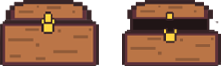
\includegraphics[width=0.3\linewidth]{./images/chest.png}
		\caption{Use Case diagram}
		\label{fig:usecase}
	\end{figure}
	\subsection{Varázsfőzet}
	A játékban elérhető két főzet és két fegyver. A piros ital növeli az életerőnket, míg a kék ital az ugrásunkat. A pályán egy avokádó és egy kenyér fegyver is található, ezek különböző erősségűek. 
	
	Mivel a pályán többféle varázsfőzet található, ezért a nevét, képét és a típusát egy interfészben tároltam, illetve a típust lehetséges értekeit egy unióban. Létrehoztam egy map-et, amely kulcs-érték pároknak a gyűjteménye, a kulcsok a főzetek nevei, az értékei pedig az interfészben definiált típusok. Ezzel a kialakítással könnyen lehet azonosítani az adott főzetet, amikor a játékos érintkezik egyel.
	\begin{lstlisting}[language=JavaScript]
	type PotionType = 'health' | 'jump' | 'avocado' | 'bread';
	interface Potion {
		name: string;
		sprite: string;
		type: PotionType;
	}
	const potionMap: Record<string, Potion> = {
		'potion_health': { name: 'potion_health', sprite: 'potionhealth', type: 'health' },
		'potion_jump': { name: 'potion_jump', sprite: 'potionjump', type: 'jump' },
		'avocado': {name: 'avocado', sprite: 'avocado', type: 'avocado'},
		'bread': {name: 'bread', sprite: 'bread', type: 'bread'}
	};
	}
	\end{lstlisting}
	\begin{figure}[!h]
		\centering
		
\includegraphics[width=0.2\linewidth]{./images/potions.png}
		\caption{Use Case diagram}
		\label{fig:usecase}
	\end{figure}
	\section{Karakterek létrehozása}
	A játék legfontosabb elemei a karakterek. Az ellenségek számára létrehoztam egy Enemy osztályt, illetve a karaktereket egy-egy osztályként kezeltem:
	\begin{itemize} 
		\item Player osztály
		\item Ninja osztály
		\item Hunter osztály
		\item Granny osztály
	\end{itemize}
	Az Enemy osztály ebben az esetben is a kód újrafelhasználhatósága miatt hoztam létre. Itt töltöttem be a játék funkcionalitásához elengedhetetlenen elemeket, a pályát, játékost, karaktereket és az életerőt.
	
	
	\subsection{Nagymama}
	A nagymama közepes látótávolsággal rendelkezik, lassú mozgása és nem okoz sebzést a játékos számára, azonban elvesz tőle egy élelmiszert.
	Az ellenségek megvalósításához először a követést kellett megvalósítanom, ehhez létrehoztam egy függvényt, ami a játékos és jelen esetben a nagymama karakterek közti távolságot számolja ki a Phaser.Math.Distance.Between metódus segítségével. Amennyiben a távolság kevesebb, mint 400 a függvény bizonyos műveleteket hajt végre, jelen esetben, amennyiben ütközés is történt a játékos eszköztárából eltűnik egy élelmiszer. 
	\begin{lstlisting}[language=JavaScript]
		updateActiveGranny() {
			if (!this.group.children.entries) return
			this.group.children.entries.map(m => {
				const distance = Phaser.Math.Distance.Between(
				this.deliveryboy.x, this.deliveryboy.y,
				m.body.position.x, m.body.position.y
				)  
				if (distance < 400) {
					...
					if (this.activeGranny) {
						this.game.playercontroller.setItem(-1);
						...
					}
				}
			});
		}
	\end{lstlisting}

	\subsection{Ninja}
	A ninja kis látótávolsággal rendelkezik, mozgása gyors és ha eléri a játékost kis sebzést okoz a számára.
	
	Az előbb bemutatott függvényben a távolság figyelést követően a nagymama és a ninja elkezdik követni a játékost. A követéshez egy függvényt hoztam létre, ami két paramétert vár. A követendő ellenséget, és egy logikai értéket, amit a távolság alapján igaz és hamis értékkel hívok meg. Amennyiben a függvény igaz értékkel hívódik meg az ellenség elkezdi követni a játékost a moveToObject() segítségével, valamint elindul egy animáció is. Ellenkező esetben a követés leáll és az animáció is.
	\begin{lstlisting}[language=JavaScript]
	follow(ninja: Phaser.GameObjects.GameObject | any, move: boolean){
		if(move){
			this.scene.physics.moveToObject(ninja, this.deliveryboy, 120);
			ninja.body.gameObject.anims.play("ninja_walk", true);
		}else{
			ninja.body.gameObject.anims.play("ninja_walk", false);
			ninja.body.velocity.setTo(0, 0);
		}
	}
	\end{lstlisting}
	\subsection{Vadász}
	A vadász nagy látótávolsággal rendelkezik, és a fegyvere segítségével nagy sebzést okoz a játékos száméra.
	
	A vadász nem mozog csak támadja a játékost, amit egy függvényben valósítottam meg. Először létrehoztam egy lövedékcsoportot, amiknek különböző paramétereket adtam. Az ütközést itt is kezelni kellett a lövedékkel, ahol ütközés esetében az ellenség életereje csökken. Az vadász 2 másodpercenként lő, amihez figyelni kell a játékmenet aktuális idejét és a utolsó tüzelés óta eltelt időt. Amikor letelt a 2 másodperc a lövés elindul.
	\begin{lstlisting}[language=JavaScript]
	shooting(m: Phaser.GameObjects.GameObject | any) {
		let shoot = this.scene.physics.add.group({ 
			frameQuantity: 1,
			active: false,
			visible: false,
			allowDrag: false,
			key: "gunshot" });
		this.scene.physics.add.collider(this.deliveryboy, shoot, this.hitPlayer, undefined, this)
		const st = shoot.getFirstDead(false);
		if (this.scene.time.now > this.nextFire) {
			this.nextFire = this.scene.time.now + 2000;
			m.anims.play("hunter_shoot", true);
			if (st) {
				st.body.reset(m.body.position.x, m.body.position.y);
				st.setActive(true);
				st.setVisible(true);
				this.scene.physics.moveTo(st, this.deliveryboy.x, this.deliveryboy.y, 900)
				}
			}
	}
	\end{lstlisting}
	\subsection{Pizzafutár}
	A játékos egy pizzafutárt irányít, aki mozog, támad és pizzát készít a játékmenet során.
	
	A játékos képes messzire is támadni, aminek a logikája hasonló a vadász támadásához, de képes közelre is támadni. A közeli támadáshoz egy hitEnemy függvényt köztam létre, ami először beállítja az aktív ellenséget, majd a életcsíkot az aktuális élete alapján. Ezt követően egy eseménykezelő figyeli, hogy a játékos a megfelelő ellenségre kattintott-e, amennyiben igen akkor az ellenség életerejét és az életcsíkját elkezdi csökkenteni a függvény. Amennyiben az ellenség élete elfogyott törlődik és a játékos tapasztalati pontjai nőnek.
	\begin{lstlisting}[language=JavaScript]
		hitEnemy(enemy: Phaser.Physics.Arcade.Sprite | undefined) {
			if (!enemy) return
			this.activeHitNinja = enemy;
			let size = enemy!.getData('health') / 500;
			this.hb!.setScale(size, 0.2)
			if (!this.control) {
				this.activeHitNinja!.setInteractive().on('pointerup', () => {
					if(this.activeHitNinja?.body.touching.left || this.activeHitNinja?.body.touching.right){
						this.activeHitNinja!.setData('health', this.activeHitNinja!.getData('health') - 20)
						this.hb!.setScale(size, 0.2)
						size -= 0.04;
						if (this.activeHitNinja!.getData('health') <= 0) {
							this.activeHitNinja!.destroy();
							this.hb!.setScale(0, 0)
							this.activeHitNinja = undefined;
							this.game.playercontroller?.setTp(1);
							this.control = false;
						}
					}
				})
				this.control = true;
			}
		}
	\end{lstlisting}
	\section{Firebase létrehozása}
	Ahhoz, hogy egy már meglévő játékot összeköthessem a Firebase-el, először létre kellett hoznom egy Firebase projektet a Firebase webhelyén. A projekt létrehozása után egy konfigurációs kódot kaptam, amelyet be illesztettem az alkalmazásba a FirebaseConfig fájlba. Miután a Firebase SDK telepítése befejeződött, az alkalmazásom sikeresen kapcsolódott a Firebase-hez.
	
	\subsection{Bejelentkezés és regisztráció}
	A Firebase segítségével a bejelentkezés és a regisztráció viszonylag egyszerű módon történik az alábbi függvények segítségével.
	
	\begin{lstlisting}[language=JavaScript]
	firebase.auth().createUserWithEmailAndPassword(email, password)
	.then((userCredential) => {
		...
	})
	.catch((error) => {
		...
	});
	\end{lstlisting}
	\begin{lstlisting}[language=JavaScript]
		firebase.auth().signInWithEmailAndPassword(email, password)
		.then((userCredential) => {
			...
		})
		.catch((error) => {
			...
		});
	\end{lstlisting}
	\subsection{Scoreboard}
	A játékom során a Firestore adatbázist használtam az adatok kezelésére. Az addDataToFirebase függvény használatával adatokat küldtem az adatbázisba, amihez az addDoc függvény létrehoz egy új dokumentumot a kollekcióban, amely tartalmazza a felhasználó nevét és pontszámát.
	\begin{lstlisting}[language=JavaScript]
	function addDataToFirebase() {
		...
		addDoc(collection(db, "users"), {name: user, points: Number(tppont)})
	}
	\end{lstlisting}
	Az adatok megjelenítésére a getDataFromFirebase függvényt használtam, ami az adatbázisból összegyűjti a top 10 pontszámot elért felhasználó nevét és pontszámát, majd ezekből generál egy HTML táblázatot, ami megjeleníti az adatokat.

	\begin{lstlisting}[language=JavaScript]
	async function getDataFromFirebase(){
		const db = getFirestore();
		const colRef = collection(db, "users");
		const docsSnap = await getDocs(query(colRef, orderBy("points","desc"), limit(10)));
		docsSnap.forEach(doc => {
			let data = doc.data();
			let row  = `<tr> <td>${data.name}</td><td>${data.points}</td> </tr>`;
			let table = document.getElementById('table')
			table!.innerHTML += row
		})
	}
	\end{lstlisting}

	\chapter{A játék tesztelése}
	
	\section{Használhatósági teszt}
	A használhatósági tesztelés egy termék vagy szolgáltatás használhatóságát és hatékonyságát méri a felhasználó interakcióinak megfigyelésével. A tesztelés célja, hogy mérjék a felhasználói elégedettséget, felderítsék az esetleges hibákat és nehézségeket, valamint ezeknek az okait. A teszt során a résztvevőket feladatokra kérik, melyek elvégzése közben kipróbálják az adott terméket, majd a használat közbeni tapasztalatokat elemzik és értékelik.
	
	A tesztelést megelőzően készítettem egy tutoriál pályát, ahol különböző instrukciókat adtam a felhasználóknak, a játék teljesítését illetőleg. A használhatósági tesztelést el lehet végezni élőben, de akár online űrlapok segítségével. Én az utóbbit választottam a szakdolgozatom tesztelése során. A teszteléshez elkészítettem egy űrlapot a Google online szolgáltatásának a segítségével, ahol különböző kérdéseket tettem fel a kitöltők számára.
	
	A kérdéseket három csoportra osztottam, elsőként a demográfiai és játék szokási kérdéseket tettem fel. A tesztelésben 28 kitöltő vett részt, akik közül 17 férfi és 11 nő volt. Az eredményekből kiderült, hogy a legtöbb kitöltő napi 1-5 órát játszik játékokkal, míg 17\% egyáltalán nem játszik. A résztvevők több mint fele 19-25 év közötti volt, de a kitöltés során 18-60 év között minden korosztályt sikerült elérni. A kitöltők több mint fele rendszeresen játszik online játékokkal. Azok a kitöltők, akik napi egynél több órát játszanak leginkább a számítógépes játékokat preferálják, ezt követte a mobilos, konzolos végül a webes játékok.
	
	\begin{figure}[!h]
		\centering
		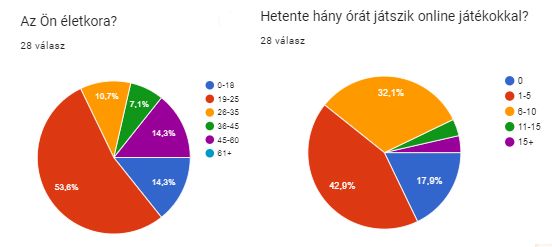
\includegraphics[width=1\linewidth]{./images/diagrams.jpg}
		\caption{Use Case diagram}
		\label{fig:usecase}
	\end{figure}	
	
	A következő csoport kérdései a menü használhatóságára tért ki. A kitöltőknek a játék menüjének elemeinek a neve és elrendezése egyértelmű volt a kitöltők 98\%-ának, azonban a menü színösszeállítása 2 kitöltőnek nem tetszett. A játékszabályokat 60\%-a a részvetőknek nagyon érhetőnek találta, 30\%-nak figyelmesebb elolvasásra volt szüksége, míg a többi kitöltőnek többszöri átolvasásra volt szüksége. 
	\begin{figure}[!h]
		\centering
		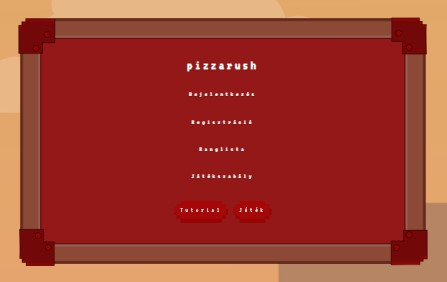
\includegraphics[width=0.8\linewidth]{./images/menu.jpg}
		\caption{Use Case diagram}
		\label{fig:usecase}
	\end{figure}
	
	A menü megtekintése után arra kértem a kitöltőket, hogy játsszák végig a tutorial pályát. Az utasításokat a felhasználók egyértelműnek tekintettették, valamint a játékmenetet is. Ezen felül a kitöltők 80\%-a tartotta érdekesnek is a játékmenetet, és csupán csak 1 embernek okozott nehézséget a megtanulása. A ninja és a vadász legyőzésének nehézsége megosztó volt a kitöltők számára, a kitöltők fele szerint nehéz volt a legyőzésük, míg a másik fele szerint egyszerű. A mama elkerülését inkább nehéznek ítélték meg a kitöltők. A grafikai elemeket mindenki kiválónak minősítette. A kitöltők közül 22 ember gondolja azt, hogy a játék érdekes, valamint a továbbfejlesztésre érdemes.
	
	Összességében a játék jól teljesített a használhatósági teszten, azonban akadt olyan felhasználó, akinek nehézséget okozott a játék irányítása. A játékmenet érdekessége, valamint a grafikai elemekre adott visszajelzés nagyon pozitív volt, ezáltal a játék javasolt a továbbfejlesztésre, ezzel is kiküszöbölve azokat a hibákat amiket okozott néhány felhasználó számára.

	\section{A fejlesztés nehézségei}
	\subsection{Nagymama}
	A használhatósági teszt során a nagymama, a játékosokat horizontálisan és vertikálisan is követte, ami sok felhasználó számára gondot okozott, ugyanis a kikerülése szinte lehetetlen volt a számukra. A kitöltős eredményeképp ezt módosítottam csak horizontális követésre az alábbi kód segítségével:
	
	\begin{lstlisting}[language=JavaScript]
		m.body.velocity.x = 60 * Math.sign(this.deliveryboy.x - m.body.position.x);
	\end{lstlisting}
	A Math.sign() függvény kiszámolja a pizzafutár a nagymama baloldalán vagy jobb oldalén helyezkedik el és ez alapján mozgatja a nagymamát az x tengelyén. Az első megoldásomkor a moveToObject() függvényt használtam ami a Phaser-nek egy beépített függvénye, ami útvonalat hoz létre két objektum között.
	
	\subsection{Vadász}
	
	
	\subsection{Ninja}
	Az életcsík kezelése során több nehézségbe is ütköztem. Az első ilyen, hogy mindegyik ellenségnek tárolni kellett az életét, majd ezt frissíteni a sebzést követően. A Phaser-nek van egy beépített függvénye, ami lehetővé teszi, hogy adatokat tároljunk és nyerjünk ki az objektumokból. Ez a getData() és setData() függvény, ami az adott kulcshoz tartozó adatot adja vissza. Az ellenségek létrehozásakor a getData() fügvénnyel beállítottam mindegyik életerejét, majd támadáskor a setData() függvénnyel módosítottam azokat.
	
	A következő nehézség a élet megjelenítése volt az ellenségek felett. A megoldást végül egy grafikai objektummal oldottam meg, ami mindig kirajzolódik, amint a játékos megfelelő távolságra van az ellenségtől. Azt, hogy a támadással módosuljon az objektum mérete, a Phaser setScale() metódusával csökkentettem, ami szabad skálázást biztosít.
	
	\subsection{Ládák}
	A ládák kivitelezésekkor az animációk megjelenítése volt a legnehezebb. Az első animáció amit próbáltam, az volt, hogy a képernyő sarkában kússzanak a ládában található élelmiszerek, azonban ez több nehézséget okozott és nem is nézett ki a megfelelően. Ezt követően megvalósítottam a jelenleg is működő animációt, amiben az élelmiszerek feldobónak, majd eltűnnek. Az animáció elkészítése után előállít egy hiba, amint az élelmiszerek hozzáértek a játékoshoz, elkezdtek újratöltődni, ezáltal rengetek élelmiszert gyűjtött be a játékos egyetlen láda kinyitásával. A hibát az okozta, hogy az élelmiszereket a láda osztályban hoztam létre és a kollíziót erre is érzékelte. A megoldást azt adta, hogy a ckeckCollision értéket hamisra kellett állítanom, ezáltal az élelmiszerekkel való érintkezés figyeli a játék.
	
	
	
	\chapter{Összegzés}
	A tervezési fázisban leírt célokat és a játék minden elemét sikeresen megvalósítottam. A fejlesztési folyamatok az elején nem voltak zökkenőmentesek, ugyanis még sosem készítettem játékot, de az elér eredménnyel elégett vagyok.
	\section{Tapasztalatok}
	A játék elkészítése során számos új ismeretre tettem szert, amit bízok benne, hogy a jövőben is alkalmazni tudom. Először is sokat tanultam a programozásról, különösen a TypeScript és Phaser keretrendszer használatáról. Megtanultam hogyan kell használni a különböző osztályokat és metódusokat a játék logikájának létrehozáshoz, illetve hogyan kell ezeket összekapcsolni a játék grafikai elemeivel. Többek között  megtapasztaltam, hogyan kell egy játékot tervezni és felépíteni úgy, hogy az szórakoztató legyen a játékosok számára.
	
	\section{További fejlesztési lehetőségek}
	Annak ellenére, hogy a célkitűzés során minden funkció belekerült a játékba számos fejlesztési lehetőség rejlik még benne:
	\begin{itemize} 
		\item A játék élményt nagyban növelné, ha a pályára felkerülnének még extra elemek, esetleg indák, egyéb akadályok.
		\item A játékos guggolásának a megvalósítása, ezáltal bekerülnének ilyen akadályok is a pályára.
		\item Több varázsital bevezetése, például a ninjához erősebb ütés.
		\item Különböző hangeffektek megvalósítása.
		\item Még több animáció és vizuális effekt hozzáadása a játékhoz.
		\item A tutoriál pályán lévő utasítások kibővítése, hogy még egyértelműbb legyen a felhasználók számára, esetleg ezek az utasításoknak a megjelenítésén való változtatás.
		\item Könnyű, közepes és nehéz játékmód bevezetése.
	\end{itemize}
	\chapter{Függelék}
	
	\section{A program forráskódja}
	A függelékbe kerülhetnek a hosszú táblázatok, vagy mondjuk egy programlista:
	% A verbatim kornyezet hasznalatanal ügyeljünk rá, hogy az editor a szóközöjket át ne írja tab karakterekre!
	\begin{verbatim}
		while (ujkmodosito[i]<0)
		{
			if (ujkmodosito[i]+kegyenletes[i]<0)
			{
				j=i+1;
				while (j<14)
				if (kegyenletes[i]+ujkmodosito[j]>-1) break;
				else j++;
				temp=ujkmodosito[j];
				for (l=i;l<j;l++) ujkmodosito[l+1]=ujkmodosito[l];
				ujkmodosito[i]=temp;
			}
			i++;
		}
	\end{verbatim}
	\begin{figure}[!h]
		\centering
		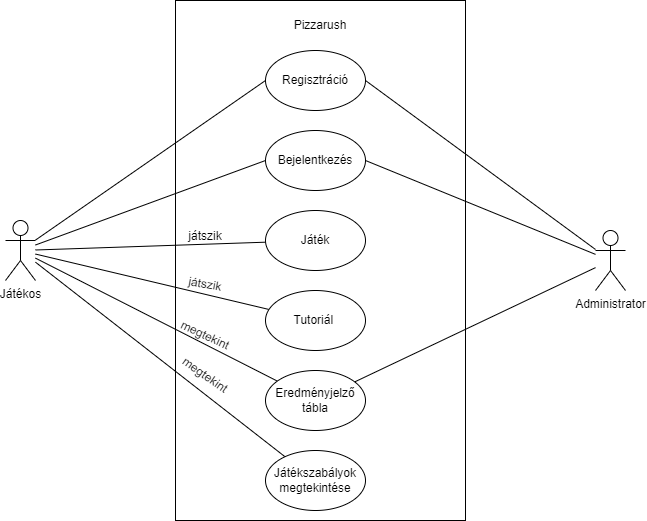
\includegraphics[width=1\linewidth]{./images/usecase.png}
		\caption{Use Case diagram}
		\label{fig:usecase}
	\end{figure}

	\begin{figure}[!h]
		\centering
		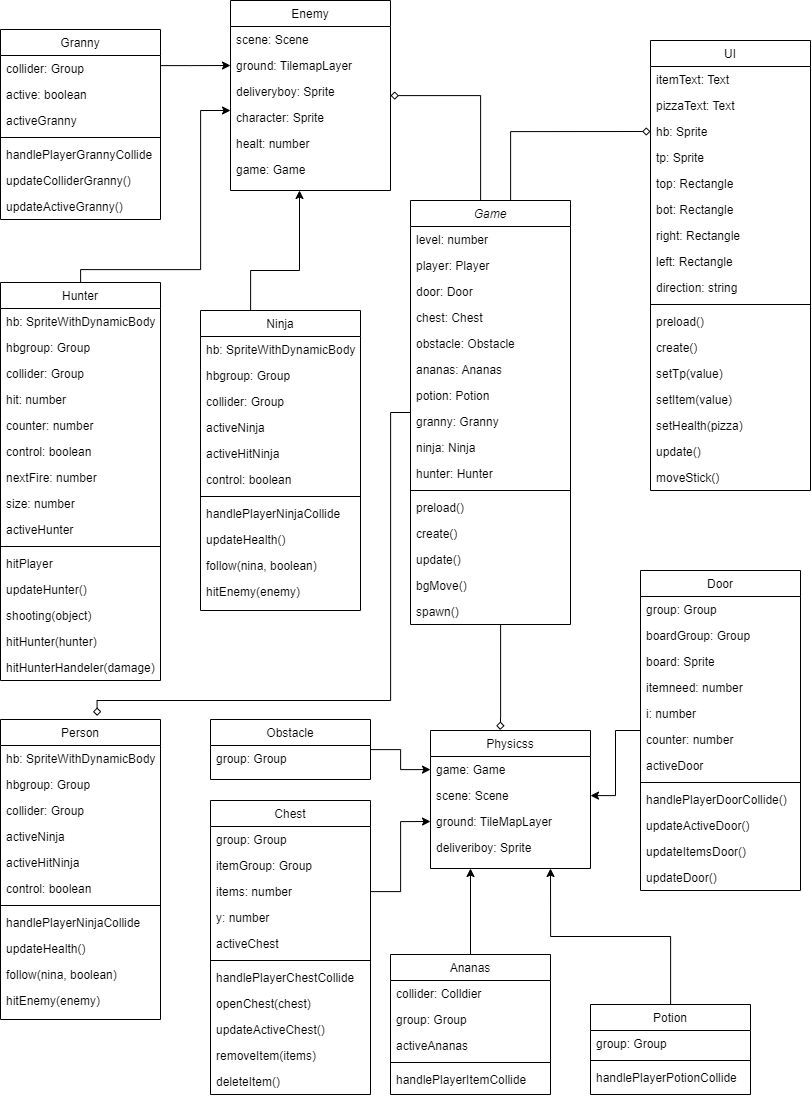
\includegraphics[width=1\linewidth]{./images/class.png}
		\caption{Class diagram}
		\label{fig:class}
	\end{figure}
	
	\chapter*{Nyilatkozat}
	%Egy üres sort adunk a tartalomjegyzékhez:
	\addtocontents{toc}{\ }
	\addcontentsline{toc}{section}{Nyilatkozat}
	%\hspace{\parindent}
	
	% A nyilatkozat szövege más titkos és nem titkos dolgozatok esetében.
	% Csak az egyik tipusú myilatokzatnak kell a dolgozatban szerepelni
	% A ponok helyére az adatok értelemszerűen behelyettesídendők es
	% a szakdolgozat /diplomamunka szo megfeleloen kivalasztando.
	
	
	%A nyilatkozat szövege TITKOSNAK NEM MINŐSÍTETT dolgozatban a következő:
	%A pontokkal jelölt szövegrészek értelemszerűen a szövegszerkesztőben és
	%nem kézzel helyettesítendők:
	
	\noindent
	Alulírott \makebox[4cm]{\dotfill} szakos hallgató, kijelentem, hogy a dolgozatomat a Szegedi Tudományegyetem, Informatikai Intézet \makebox[4cm]{\dotfill} Tanszékén készítettem, \makebox[4cm]{\dotfill} diploma megszerzése érdekében.
	
	Kijelentem, hogy a dolgozatot más szakon korábban nem védtem meg, saját munkám eredménye, és csak a hivatkozott forrásokat (szakirodalom, eszközök, stb.) használtam fel.
	
	Tudomásul veszem, hogy szakdolgozatomat / diplomamunkámat a Szegedi Tudományegyetem Informatikai Intézet könyvtárában, a helyben olvasható könyvek között helyezik el.
	
	\vspace*{2cm}
	
	\begin{tabular}{lc}
		Szeged, \today\
		\hspace{2cm} & \makebox[6cm]{\dotfill} \\
		& aláírás \\
	\end{tabular}
	
	
	\vspace*{4cm}
	
	%A nyilatkozat szövege TITKOSNAK MINŐSÍTETT dolgozatban a következő:
	
	\noindent
	Alulírott \makebox[4cm]{\dotfill} szakos hallgató, kijelentem, hogy a dolgozatomat a Szegedi Tudományegyetem, Informatikai Intézet \makebox[4cm]{\dotfill} Tanszékén készítettem, \makebox[4cm]{\dotfill} diploma megszerzése érdekében.
	
	Kijelentem, hogy a dolgozatot más szakon korábban nem védtem meg, saját munkám eredménye, és csak a hivatkozott forrásokat (szakirodalom, eszközök, stb.) használtam fel.
	
	Tudomásul veszem, hogy szakdolgozatomat / diplomamunkámat a TVSZ 4. sz. mellékletében leírtak szerint kezelik.
	
	\vspace*{2cm}
	
	\begin{tabular}{lc}
		Szeged, \today\
		\hspace{2cm} & \makebox[6cm]{\dotfill} \\
		& aláírás \\
	\end{tabular}
	
	
	
	
	
	\chapter*{Köszönetnyilvánítás}
	\addcontentsline{toc}{section}{Köszönetnyilvánítás}
	
	Ezúton szeretnék köszönetet mondani \textbf{X. Y-nak} ezért és ezért \ldots
	
	
	%% Az itrodalomjegyzek keszitheto a BibTeX segedprogrammal:
	%\bibliography{diploma}
	%\bibliographystyle{plain}
	
	%VAGY "kézzel" a következő módon:
	
	\begin{thebibliography}{9}
		%10-nél kevesebb hivatkozás esetén
		
		%\begin{thebibliography}{99}
		% 10-nél több hivatkozás esetén
		
		\addcontentsline{toc}{section}{Irodalomjegyzék}
		
		%Elso szerzok vezetekneve alapjan ábécérendben rendezve.
		
		\bibitem{Gischer}
		Wikipédia: korai története a videójátékoknak
		\emph{\url{https://en.wikipedia.org/wiki/Early_history_of_video_games}}
		Internet, 2023
		
		\bibitem{Gischer}
		Exploding topics: játékosok kutatása
		\emph{\url{https://explodingtopics.com/blog/number-of-gamers}}
		Internet, 2023
		
		\bibitem{Gischer}
		Wikipedia: HTML5 
		\emph{https://en.wikipedia.org/wiki/HTML5}
		Internet, 2023
		
		\bibitem{Gischer}
		MDN Web Docs: HTML5
		\emph{https://developer.mozilla.org/en-US/docs/Glossary/HTML5}
		Internet, 2023
		
		\bibitem{Gischer}
		MDN Web Docs: JavaScript Oktatóanyagok
		\emph{https://developer.mozilla.org/en-US/docs/Web/JavaScript?retiredLocale=hu}
		Internet, 2023
		
		\bibitem{Gischer}
		Wikipedia: TypeScript
		\emph{https://en.wikipedia.org/wiki/TypeScript}
		Internet, 2023
		
		\bibitem{Gischer}
		Phaser, hivatalos weboldal
		\emph{https://phaser.io/}
		Internet, 2023
		
		\bibitem{Gischer}
		MDN Web Docs: Tiles és TileMap
		\emph{https://developer.mozilla.org/en-US/docs/Games/Techniques/Tilemaps}
		Internet, 2023
		
		\bibitem{Gischer}
		Git: hivatalos weboldal
		\emph{https://git-scm.com/}
		Internet, 2023
		

		
		%folyóirat cikk: szerzok(k), a folyóirat neve kiemelve,
		%az evfolyam felkoveren, zarojelben az evszam, vegul az oldalszamok es pont.
		\bibitem{Gischer}
		J. L. Gischer,
		The equational theory of pomsets.
		\emph{Theoret. Comput. Sci.}, \textbf{61}(1988), 199--224.
		
		%könyv (szerzo(k), a könyv neve kiemelve, utana a kiado, a kiado szekhelye, az evszam es pont.)
		\bibitem{Pin}
		J.-E. Pin,
		\emph{Varieties of Formal Languages},
		Plenum Publishing Corp., New York, 1986.
		
		
		
		
		
	\end{thebibliography}
	
	
	
	
\end{document}
